\chapter{Superposition}
\label{c:super}

Superposition is the insertion of elements into a lattice after the lattice has been created by the 
\vn{expand} function. Superposition is beneficial for various purposes. A common use of superposition is to
insert \vn{marker} elements within other elements. For example, placing a marker element in the middle
of a quadrupole. 
Another use case is when the field in some region is due to the overlap of several
elements. For example, a quadrupole magnet inside a larger solenoid magnet.

%-----------------------------------------------------------------------------
\section{Superposition on a Drift}
\label{s:super.fund}

\begin{figure}[tb]
  \centering 
  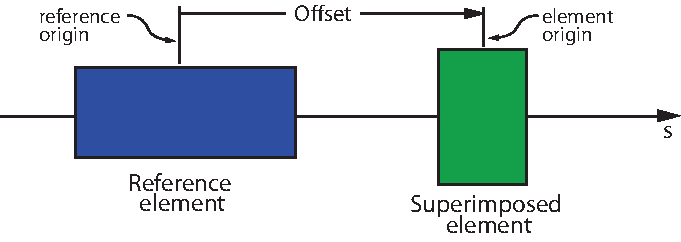
\includegraphics[width=0.8\textwidth]{superimpose-positioning.pdf} 
  \caption[Superposition Offset.]{
The superposition \vn{offset} is the longitudinal $s$-distance from the origin point of the
reference element to the origin point of the element being superimposed.
  }
  \label{f:superimpose}
\end{figure}

A simple example illustrates how superposition works (also see section \sref{s:lord.slave}):
\begin{example}
  using AcceleratorLattice
  @ele dd = Drift(L = 12)
  @ele bb = BeginningEle(species_ref = species("proton"), pc_ref = 1e11)
  @ele ss = Solenoid(L = 1)
  zline = beamline("z", [bb, dd])
  lat = expand("lat", zline)

  ref_ele = find_eles(lat, "dd")
  superimpose!(ss, ref_ele, offset = 0.2)
\end{example}
Before superposition, branch 1 of lattice \vn{lat} looks like
\begin{example}
  Branch 1: "z"  geometry => open             L           s      s_downstream
    1  "bb"           BeginningEle        0.000000    0.000000 ->    0.000000
    2  "dd"           Drift              12.000000    0.000000 ->   12.000000
    3  "end_ele"      Marker              0.000000   12.000000 ->   12.000000
\end{example}

The \vn{superimpose!} function has the signature
\begin{example}
  function superimpose!(super_ele::Ele, ref::T; 
          ele_origin::BodyLocationSwitch = b_center, offset::Real = 0, 
          ref_origin::BodyLocationSwitch = b_center, wrap::Bool = true) 
          where {E <: Ele, T <: Union{Branch, Ele, Vector{Branch}, Vector{E}}}
\end{example}
The superimpose

statement inserts a copy of the element \vn{ss} in the lattice. 




After insertion, branch 1 looks like:
\begin{example}
  Branch 1: "z"  geometry => open             L           s      s_downstream
    1  "bb"           BeginningEle        0.000000    0.000000 ->    0.000000
    2  "dd!1"         Drift               5.700000    0.000000 ->    5.700000
    3  "ss"           Solenoid            1.000000    5.700000 ->    6.700000
    4  "dd!2"         Drift               5.300000    6.700000 ->   12.000000
    5  "end_ele"      Marker              0.000000   12.000000 ->   12.000000
\end{example}
The insertion of the \vn{ss} copy is within the \vn{drift} named \vn{dd}. The position

With superpositions, \vn{Drift} elements are handled differently from other elements. This is done
to simplify the bookkeeping code. T



Rules:
\begin{itemize}
%
\item
The \vn{super_ele} element cannot be a \vn{Drift}.
%
\item
%
The \vn{bookkeeper!} function must be called after any superpositions or 
%
\end{itemize}


Branch 1: "z"  geometry => open                 L           s       s_downstream
      1  "bb"           BeginningEle        0.000000    0.000000 ->    0.000000
      2  "dd"           Drift              12.000000    0.000000 ->   12.000000
      3  "end_ele"      Marker              0.000000   12.000000 ->   12.000000


\begin{example}
  using AcceleratorLattice
  @ele qq = Quadrupole(L = 4)
  @ele dd = Drift(L = 12)
  @ele ss = Solenoid(L = 1)
  @ele bb = BeginningEle(species_ref = species("proton"), pc_ref = 1e11)
  zline = beamline("z", [bb, qq, dd])
  lat = expand("lat", zline)

  ref_ele = find_eles (lat, "dd")
  superimpose!(ss, ref_ele, offset = 0.2)
\end{example}

parameter of element \vn{S} superimposes \vn{S} over the lattice \vn{(Q,
D)}. The placement of \vn{S} is such that the beginning of \vn{S} is coincident with the center of
\vn{Q} (this is is explained in more detail below). Additionally, a marker \vn{M} is superimposed at
a distance of +1~meter from the center of \vn{S}. The tracking part of the lattice
(\sref{s:lord.slave}) looks like:
\begin{example}
        Element   Key         Length  Total     
  1)    Q{\#}1       Quadrupole   2        2
  2)    Q{\B}S       Sol_quad     2        4
  3)    S{\#}1       Solenoid     3        7
  4)    M         Marker       0      
  4)    S{\#}2       Solenoid     3       10
  5)    D{\#}2       Drift        4       14
\end{example}
What \bmad has done is to split the original elements \vn{(Q, D)} at the edges of \vn{S} and then
\vn{S} was split where \vn{M} is inserted. The first element in the lattice, \vn{Q\#1}, is the part
of \vn{Q} that is outside of \vn{S}. Since this is only part of \vn{Q}, \bmad has put a \vn{\#1} in
the name so that there will be no confusion. (a single \vn{\#} has no special meaning other than the
fact that \bmad uses it for mangling names. This is opposed to a double \vn{\#\#} which is used to
denote the $N$\Th instance of an element (\sref{s:ele.match}). The next element, \vn{Q{\B}S}, is the
part of \vn{Q} that is inside \vn{S}. \vn{Q{\B}S} is a combination solenoid/quadrupole element as
one would expect. \vn{S{\#}1} is the part of \vn{S} that is outside \vn{Q} but before \vn{M}. This
element is just a solenoid. Next comes \vn{M}, \vn{S{\#}1}, and finally \vn{D\#2} is the rest of the
drift outside \vn{S}.

In the above example, \vn{Q} and \vn{S} will be \vn{super_lord} elements (\vn{s:lord.slave}) and
four elements in the tracking part of the lattice will be \vn{super_slave} elements. This is
illustrated in \fig{f:super.ex}B.

Notice that the name chosen for the \vn{sol_quad} element \vn{Q{\B}S} is dependent upon what is
being superimposed upon what. If \vn{Q} had been superimposed upon \vn{S} then the name would have
been \vn{S{\B}Q}.

When \bmad sets the element class for elements created from superpositions, \bmad will set the class
of the element to something other than an \vn{em_field} element (\sref{s:em.field}) if possible. If
no other possibilities exist, \bmad will use \vn{em_field}. For example, a \vn{quadrupole}
superimposed with a \vn{solenoid} will produce a \vn{sol_quad} \vn{super_slave} element but a
\vn{solenoid} superimposed with a \vn{rfcavity} element will produce an \vn{em_field} element since
there is no other class of element that can simultaneously handle solenoid and RF fields. An
\vn{em_field} \vn{super_slave} element will also be created if any of the superimposing elements 
have a non-zero orientation (\sref{s:offset}) since it is not, in general, possible to construct a slave
element that properly mimics the effect of a non-zero orientation.



With the lattice broken up like this \bmad has constructed something that can be easily
analyzed. However, the original elements \vn{Q} and \vn{S} still exist within the lord section of
the lattice. \bmad has bookkeeping routines so that if a change is made to the \vn{Q} or \vn{S}
elements then these changes can get propagated to the corresponding slaves. It does not matter which
element is superimposed. Thus, in the above example, \vn{S} could have been put in the Beam Line
(with a drift before it) and \vn{Q} could then have been superimposed on top and the result would
have been the same (except that the split elements could have different names).

If an element has zero length (for example, a \vn{marker} element), is superimposed, or is
superimposed upon, then the element will remain in the tracking part of the lattice and there will
be no corresponding lord element. See \fig{f:super.ex}.
 
Superimpose syntax:
\begin{example}
  Q: quad, superimpose, ...       ! Superimpose element Q.
  Q: quad, superimpose = T, ...   ! Same as above.
  Q: quad, ...                    ! First define element Q ...
  Q[superimpose] = T              !   ... and then superimpose.
  Q[superimpose] = F              ! Suppress superposition.
\end{example}
Superposition happens at the end of parsing so the last set of the \vn{superimpose} for an element
will override previous settings. 

It is also possible to superimpose an element using the \vn{superimpose} command which has the
syntax:
\begin{example}
  superimpose, element = <ele-name>, ...
\end{example}
With the same optional superposition parameters (\vn{ref}, \vn{offset}, etc.) given below.
Example:
\begin{example}
  superimpose, element = Q1, ref = B12, offset = 1.3, 
                               ele_origin = beginning, ref_origin = end
\end{example}
Note: Superposition using the superimpose statement allows superimposing the same element with
multiple reference elements and/or multiple offsets. The drawback is that superposition using the
superimpose statement may not be switched off later in the lattice file.

The placement of a superimposed element is illustrated in \fig{f:superimpose}. The placement of a
superimposed element is determined by three factors: An origin point on the superimposed element, an
origin point on the reference element, and an offset between the points. The parameters that
determine these three quantities are:
\index{ref}\index{offset}
\index{ref_origin}\index{ele_origin}
\begin{example}
  create_jumbo_slave = <Logical>     ! See \sref{s:jumbo.slave}
  wrap_superimpose   = <Logical>     ! Wrap if element extends past lattice ends?
  ref          = <lattice_element>
  offset       = <length>            ! default = 0
  ele_origin   = <origin_location>   ! Origin pt on element.
  ref_origin   = <origin_location>   ! Origin pt on ref element.
\end{example}
\vn{ref} sets the reference element. If \vn{ref} is not present then the start of the lattice is
used (more precisely, the start of branch 0 (\sref{s:branch.def})). Wild card characters
(\sref{s:ele.match} can be used with \vn{ref}. If \vn{ref} matches to multiple elements (which may
also happen without wild card characters if there are multiple elements with the name given by
\vn{ref}) in the lattice a superposition will be done, one for each match.

The location of the origin points are determined by the setting of \vn{ele_origin} and
\vn{ref_origin}.  The possible settings for these parameters are
\begin{example}
  beginning       ! Beginning (upstream) edge of element
  center          ! Center of element. Default.
  end             ! End (downstream) edge of element
\end{example}
\vn{center} is the default setting. \vn{Offset} is the longitudinal offset of the origin 
of the element being superimposed relative
to the origin of the reference element. The default offset is zero.  
A positive offset moves the element being superimposed in the \vn{downstream} direction if
the reference element has a normal longitudinal \vn{orientation} (\sref{s:ele.reverse}) and
vice versa for the reference element has a reversed longitudinal orientation.

Note: There is an old syntax, deprecated but still supported for now, where the origin points were
specified by the appearance of:
\begin{example}
  ele_beginning         ! Old syntax. Do not use.
  ele_center            ! Old syntax. Do not use.
  ele_end               ! Old syntax. Do not use.
  ref_beginning         ! Old syntax. Do not use.
  ref_center            ! Old syntax. Do not use.
  ref_end               ! Old syntax. Do not use.
\end{example}
For example, ``ele_origin = beginning'' in the old syntax would be ``ele_beginning''.

\index{drift}
\index{overlay}\index{group}\index{girder}
The element begin superimposed may be any type of element except \vn{drift}, \vn{group},
\vn{overlay}, and \vn{girder} control elements. The reference element used to position a
superimposed element may be a \vn{group} or \vn{overlay} element as long as the \vn{group} or
\vn{overlay} controls the parameters of exactly one element. In this case, the controlled element is
used as the reference element.

\index{geometry}\index{open}
By default, a superimposed element that extends beyond either end of the lattice will be wrapped
around so part of the element will be at the beginning of the lattice and part of the element will
be at the end. For consistency's sake, this is done even if the \vn{geometry} is set to \vn{open}
(for example, it is sometimes convenient to treat a circular lattice as linear). Example:
\begin{example}
  d: drift, l = 10
  q: quad, l = 4, superimpose, offset = 1
  machine: line = (d)
  use, machine
\end{example}
The lattice will have five elements in the tracking section:
\begin{example}
        Element    Key             Length
  0)    BEGINNING  Beginning_ele   0
  1)    Q{\#}2        Quadrupole      3   ! Slave representing beginning of Q element
  2)    D{\#}1        Drift           6
  3)    Q{\#}1        Quadrupole      1   ! Slave representing end of Q element
  4)    END        Marker          0
\end{example}
And the lord section of the lattice will have the element \vn{Q}. 

To not wrap an element that is being superimposed, set the \vn{wrap_superimpose} logical to \vn{False}.
Following the above example, if the definition of\vn{q} is extended by adding \vn{wrap_superimpose}:
\begin{example}
  q: quad, l = 4, superimpose, offset = 1, wrap_superimpose = F
\end{example}
In this instance there are four elements in the tracking section:
\begin{example}
        Element    Key             Length
  0)    BEGINNING  Beginning_ele   0
  1)    Q          Quadrupole      4    
  2)    D{\#}1        Drift           7
  4)    END        Marker          0
\end{example}
And the lord section of the lattice will not have any elements.

To superimpose a zero length element ``\vn{S}'' next to a zero length element ``\vn{Z}'', and to
make sure that \vn{S} will be on the correct side of \vn{Z}, set the \vn{ref_origin} appropriately.
For example:
\begin{example}
  S1: marker, superimpose, ref = Z, ref_origin = beginning
  S2: marker, superimpose, ref = Z, ref_origin = end
  Z: marker
\end{example}
The order of the elements in the lattice will be
\begin{example}
  S1, Z, S2
\end{example}
If \vn{ref_origin} is not present or set to \vn{center}, the ordering of the elements will be
arbitrary.

If a zero length element is being superimposed at a spot where there are other zero length elements,
the general rule is that the element will be placed as close as possible to the reference element.
For example:
\begin{example}
  S1: marker, superimpose, offset = 1
  S2: marker, superimpose, offset = 1
\end{example}
In this case, after \vn{S1} is superimposed at $s = 1$ meter, the superposition of \vn{S2} will
place it as close to the reference element, which in this case is the \vn{BEGINNING} elements at $s
= 0$, as possible. Thus the final order of the superimposed elements is:
\begin{example}
  S2, S1
\end{example}
To switch the order while still superimposing \vn{S2} second one possibility is to use:
\begin{example}
  S1: marker, superimpose, offset = 1
  S2: marker, superimpose, ref = S1, ref_origin = end
\end{example}

If a superposition uses a reference element, and there are $N$ elements in the lattice with the
reference element name, there will be $N$ superpositions. For example, the following will split in
two all the quadrupoles in a lattice:
\begin{example}
  M: null_ele, superimpose, ref = quadrupole::*
\end{example}
A \vn{null_ele} (\sref{s:null.ele}) element is used here so that there is no intervening element
between split quadrupole halves as there would be if a \vn{marker} element was used.


\index{drift!superposition}\index{pipe!superposition}
When a superposition is made that overlaps a drift, the drift, not being a "real" element,
vanishes. That is, it does not get put in the lord section of the lattice.  Note that if aperture
limits (\sref{s:limit}) have been assigned to a drift, the aperture limits can ``disappear'' when
the superposition is done. Explicitly, if the exit end of a drift has been assigned aperture limits,
the limits will disappear if the superimposed element overlays the exit end of the drift. A similar
situation applies to the entrance end of a drift. If this is not desired, use a \vn{pipe} element
instead. 

To simplify bookkeeping, a drift element may not be superimposed. Additionally, since drifts can
disappear during superposition, to avoid unexpected behavior the superposition reference element may
not be the $N$\Th instance of a drift with a given name. For example, if there are a number of drift
elements in the lattice named \vn{a_drft}, the following is not allowed:
\begin{example}
  my_oct: octupole, ..., superimpose, ref = a_drft##2  ! This is an error
\end{example}

When the parameters of a super_slave are computed from the parameters of its super_lords, some types
of parameters may be ``missing''. For example, it is, in general, not possible to set appropriate
aperture parameters (\sref{s:limit}) of a super_slave if the lords of the slave have differing
aperture settings. When doing calculations, \bmad will use the corresponding parameters stored in
the lord elements to correctly calculate things.

When superposition is done in a line where there is \vn{element reversal} (\sref{s:ele.reverse}),
the calculation of the placement of a superimposed element is also ``reversed'' to make the relative
placement of elements independent of any element reversal.  An example will make this clear:
\begin{example}
  d1: drift, l = 1
  d2: d1
  q1: quad, l = 0.1, superimpose, ref = d1, offset = 0.2, 
             ref_origin = beginning, ele_origin = beginning
  q2: q1, ref = d2
  p: patch, x_pitch = pi  ! Needed to separate reversed and unreversed.
  this_line: line = (d1, p, --d2)
  use, this_line
\end{example}
Since the reference element of the \vn{q2} superposition, that is \vn{d2}, is a reversed element,
\vn{q2} will be reversed and the sense of \vn{offset}, \vn{ref_origin}, and \vn{ele_origin} will be
reversed so that the position of \vn{q2} with respect to \vn{d2} will be the mirror image of the
position of \vn{q1} with respect to \vn{d1}. The tracking part of the lattice will be:
\begin{example}
  Element:           d1{\#}1    q1  d1{\#}2   d2{\#}2    q2   d2{\#}1
  Length:             0.2   0.1   0.7    0.7   0.1    0.3
  Reversed element?:   No    No    No    Yes   Yes    Yes
\end{example}

Superposition with \vn{line reflection} (\sref{s:lines.wo.arg}) works the same way as line reversal.

The \vn{no_superposition} statement (\sref{s:no.sup}) can be used to turn off superpositioning

%-----------------------------------------------------------------------------
\section{Superposition and Sub-Lines}
\label{s:super.sub.line}

Sometimes it is convenient to do simulations with only part of a lattice. The rule for how
superpositions are handled in this case is illustrated in the following example. Consider a lattice
file which defines a \vn{line} called \vn{full} which is defined by two sublines called \vn{sub1}
and \vn{sub2}:
\begin{example}
  sub1: line = {..., ele1, ...}
  sub2: line = {...}
  full: line = {sub1, sub2}
  m1: marker, superimpose, ref = ele1, offset = 3.7
  use, full
\end{example}
Now suppose you want to do a simulation using only the \vn{sub2} line. Rather than edit the original
file, one way to do this would be to create a second file which overrides the used line:
\begin{example}
  call, file = "full.bmad"
  use, sub2
\end{example}
where \vn{full.bmad} is the name of the original file. What happens to the superposition of \vn{m1}
in this case? Since \vn{m1} uses a reference element, \vn{ele1}, that is not in \vn{sub1}, \bmad
will ignore the superposition. Even though \bmad will ignore the superposition of \vn{m1} here,
\bmad will check that \vn{ele1} has been defined. If \vn{ele1} has not been defined, \bmad will
assume that there is a typographic error and issue an error message.

Notice that in this case it is important for the superposition to have an explicit reference element
since without an explicit reference element the superposition is referenced to the beginning of the
lattice. Thus, in the above example, if the superposition were written like:
\begin{example}
  m1: marker, superimpose, offset = 11.3
\end{example}
then when the \vn{full} line is used, the superposition of \vn{m1} is referenced to the beginning of
\vn{full} (which is the same as the beginning of \vn{sub1}) but when the \vn{sub2} line is used, the
superposition of \vn{m1} is referenced to the beginning of \vn{sub2} which is not the same as the
beginning of \vn{full}.

%-----------------------------------------------------------------------------
\section{Jumbo Super_Slaves}
\label{s:jumbo.slave}

The problem with the way \vn{super_slave} elements are created as discussed above is that edge
effects will not be dealt with properly when elements with non-zero fields are misaligned. When this
is important, especially at low energy, a possible remedy is to instruct \bmad to construct
``\vn{jumbo}'' super_slave elements. The general idea is to create one large \vn{super_slave} for
any set of overlapping elements. Returning to the superposition example at the start of
Section~\sref{s:super}, If the superposition of solenoid \vn{S} is modified to be
\begin{example}
  S: solenoid, l = 8, superimpose, ref = Q, ele_origin = beginning, 
               create_jumbo_slave = T
\end{example}
The result is shown in \fig{f:super.ex}C. The tracking part of the lattice will be
\begin{example}
        Element   Key         Length  Total     
  1)    Q{\B}S       Sol_quad     2        4
  2)    M         Marker       0      
  3)    S{\#}2       Solenoid     3       10
  4)    D{\#}2       Drift        4       14
\end{example}
\index{lord_pad1}\index{lord_pad2}
\vn{Q} and part of \vn{S} have been combined into a jumbo \vn{super_slave} named \vn{Q{\B}S}. Since
the \vn{super_lord} elements of a jumbo \vn{super_slave} may not completely span the slave two
parameters of each lord will be set to show the position of the lord within the slave. These two
parameters are
\begin{example}
  lord_pad1    ! offset at upstream end
  lord_pad2    ! offset at downstream end
\end{example}
\vn{lord_pad1} is the distance between the upstream edge of the jumbo \vn{super_slave} and a
\vn{super_lord}. \vn{lord_pad2} is the distance between the downstream edge of a \vn{super_lord} and
the downstream edge of the jumbo \vn{super_slave}. With the present example, the lords have the
following padding:
\begin{example}
          lord_pad1    lord_pad2
  Q            0            3
  S            2            0
\end{example}
The following rule holds for all super lords with and without jumbo slaves:
\begin{example}
  Sum of all slave lengths = lord length + lord_pad1 + lord_pad2
\end{example}

One major drawback of jumbo \vn{super_slave} elements is that the \vn{tracking_method}
(\sref{s:tkm}) will, by necessity, have to be \vn{runge_kutta}, or \vn{time_runge_kutta} and the
\vn{mat6_calc_method} (\sref{s:xfer}) will be set to \vn{tracking}.

Notice that the problem with edge effects for non-jumbo \vn{super_slave} elements only occurs when
elements with nonzero fields are superimposed on top of one another. Thus, for example, one does not
need to use jumbo elements when superimposing a \vn{marker} element.

\index{field_overlaps}
Another possible way to handle overlapping fields is to use the \vn{field_overlaps} element
parameter as discussed in \sref{s:overlap}.

%-----------------------------------------------------------------------------
\section{Changing Element Lengths when there is Superposition}
\label{s:super.length}

When a program is running, if \vn{group} (\sref{s:group}) or \vn{overlay} (\sref{s:overlay})
elements are used to vary the length of elements that are involved in superimposition, the results
are different from what would have resulted if instead the lengths of the elements where changed in
the lattice file. There are two reasons for this. First, once the lattice file has been parsed,
lattices can be ``mangled'' by adding or removing elements in a myriad of ways. This means that it
is not possible to devise a general algorithm for adjusting superimposed element lengths that
mirrors what the effect of changing the lengths in the lattice file.

Second, even if a lattice has not been mangled, an algorithm for varying lengths that is based on
the superimpose information in the lattice file could lead to unexpected results. To see this
consider the first example in Section~\sref{s:super}. If the length of \vn{S} is varied in the
lattice file, the upstream edge of \vn{S} will remain fixed at the center of \vn{Q} which means that
the length of the \vn{super_slave} element \vn{Q{\#}1} will be invariant. On the other hand, if
element \vn{S} is defined by
\begin{example}
  S: solenoid, l = 8, superimpose, offset = 6
\end{example}
This new definition of \vn{S} produces exactly the same lattice as before. However, now varying the
length of \vn{S} will result in the center of \vn{S} remaining fixed and the length of \vn{Q{\#}1}
will not be invariant with changes of the length of \vn{S}. This variation in behavior could be very
confusing since, while running a program, one could not tell by inspection of the element positions
what should happen if a length were changed.

To avoid confusion, \bmad uses a simple algorithm for varying the lengths of elements involved in
superposition: The rule is that the length of the most downstream \vn{super_slave} is varied.  With
the first example in Section~\sref{s:super}, the \vn{group} \vn{G} varying the length of \vn{Q}
defined by:
\begin{example}
  G: group = \{Q\}, var = \{l\}
\end{example}
would vary the length of \vn{Q{\B}S} which would result in an equal variation of the length of
\vn{S}. To keep the length of \vn{S} invariant while varying \vn{Q} the individual \vn{super_slave}
lengths can be varied. Example:
\begin{example}
  G2: group = \{Q{\#}1, S{\#}1:-1\}, var = \{l\}
\end{example}
The definition of \vn{G2} must be placed in the lattice file after the superpositions so that the
super slaves referred to by \vn{G2} have been created.

In the above example there is another, cleaner, way of achieving the same result by varying the
downstream edge of \vn{Q}:
\begin{example}
  G3: group = \{Q\}, var = \{end_edge\}
\end{example}

\etcetc...

*) Difference from Bmad: Superposition is always done after lattice expansion.

*) Superimposing using the same given Drift as a reference element multiple times is not allowed (unlike Bmad). 
  Instead, superimpose a Null ele at the beginning or end of the drift and then use that as the reference.
  At the end, remove the Null element

